\section{Video Vision Transformers}
\label{sec:method}

We start by summarising the recently proposed Vision Transformer~\cite{dosovitskiy_iclr_2021} in~Sec.~\ref{sec:method_background}, and then discuss two approaches for extracting tokens from video in~Sec.~\ref{sec:method_input_encoding}. Finally, we develop several transformer-based architectures for video classification in Sec.~\ref{sec:method_video_models} and~\ref{sec:method_initialisation}.


\subsection{Overview of Vision Transformers (ViT)}
\label{sec:method_background}



Vision Transformer (ViT)~\cite{dosovitskiy_iclr_2021} adapts the transformer architecture of~\cite{vaswani_neurips_2017} to process 2D images with minimal changes.
In particular, ViT extracts $N$ non-overlapping image patches, $x_i \in \mathbb{R}^{h \times w}$, %
performs a linear projection and then rasterises them into 1D tokens $z_i \in \mathbb{R}^d$. The sequence of tokens input to the following transformer encoder is
\begin{equation}
\mathbf{z} = [z_{cls}, \mathbf{E}x_1, \mathbf{E}x_2, \ldots , \mathbf{E}x_N] + \mathbf{p},
\label{eq:tokens}
\end{equation}
where the projection by $\mathbf{E}$ is equivalent to a 2D convolution.
As shown in Fig.~\ref{fig:teaser}, an optional learned classification token $z_{cls}$ is prepended to this sequence, and its representation at the final layer of the encoder serves as the final representation used by the classification layer~\cite{devlin_naacl_2019}.
In addition, a learned positional embedding, $\mathbf{p} \in \mathbb{R}^{N \times d}$, is added to the tokens to retain positional information, as the subsequent self-attention operations in the transformer are permutation invariant.
The tokens are then passed through an encoder consisting of a sequence of $L$ transformer layers.
Each layer $\ell$ comprises of Multi-Headed Self-Attention~\cite{vaswani_neurips_2017}, layer normalisation (LN)~\cite{ba_arxiv_2016}, and MLP blocks as follows:
\begin{align}
\mathbf{y}^{\ell} &= \text{MSA}(\text{LN}(\mathbf{z}^\ell)) +\mathbf{z}^\ell  \\
\mathbf{z}^{\ell + 1} &= \text{MLP}(\text{LN}(\mathbf{y}^\ell)) + \mathbf{y}^\ell.
\end{align}
The MLP consists of two linear projections separated by a GELU non-linearity~\cite{hendrycks_arxiv_2016} and the token-dimensionality, $d$, remains fixed throughout all layers.
Finally, a linear classifier is used to classify the encoded input based on $z_{cls}^L \in \mathbb{R}^d$, if it was prepended to the input, or a global average pooling of all the tokens, $\mathbf{z}^{L}$, otherwise. 


As the transformer~\cite{vaswani_neurips_2017}, which forms the basis of ViT~\cite{dosovitskiy_iclr_2021}, is a flexible architecture that can operate on any sequence of input tokens $\mathbf{z} \in \mathbb{R}^{N \times d}$, we describe strategies for tokenising videos next.

\subsection{Embedding video clips}
\label{sec:method_input_encoding}
We consider two simple %
methods for mapping a video $\mathbf{V} \in \mathbb{R}^{T \times H \times W \times C}$ to a sequence of tokens $\mathbf{\tilde{z}} \in \mathbb{R}^{n_t \times n_h \times n_w \times d}$.
We then add the positional embedding and reshape into $\mathbb{R}^{N \times d}$ to obtain $\mathbf{z}$, the input to the transformer.%



\paragraph{Uniform frame sampling} 

As illustrated in Fig.~\ref{fig:tokenizer_2d}, a straightforward method of tokenising the input video is to uniformly sample $n_t$ frames from the input video clip, embed each 2D frame independently using the same method as ViT~\cite{dosovitskiy_iclr_2021}, and concatenate all these tokens together.
Concretely, if $n_h \cdot n_w$ non-overlapping image patches are extracted from each frame, as in~\cite{dosovitskiy_iclr_2021}, then a total of $n_t \cdot n_h \cdot n_w$ tokens will be forwarded through the transformer encoder. 
Intuitively, this process may be seen as simply constructing a large 2D image to be tokenised following ViT.
We note that this is the input embedding method employed by the concurrent work of~\cite{bertasius_arxiv_2021}.


\paragraph{Tubelet embedding}
\begin{figure}
    \centering
     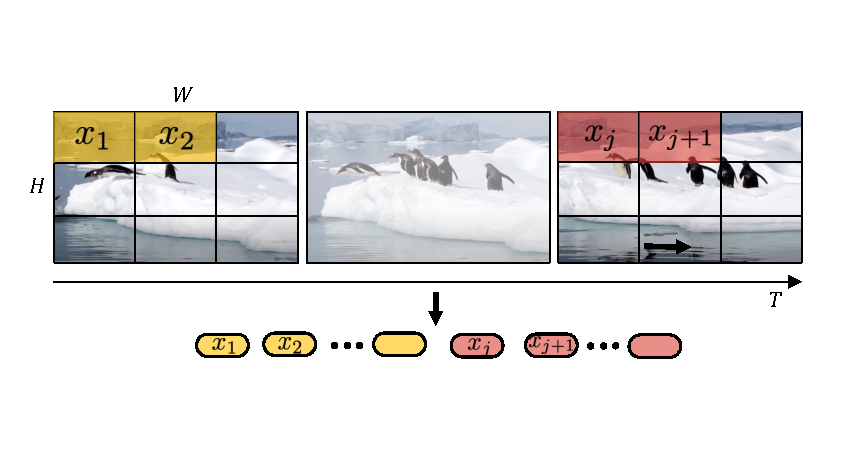
\includegraphics[width=1.0\linewidth]{figures/diagrams/Diagram-2.pdf}
    \caption{Uniform frame sampling: We simply sample $n_t$ frames, and embed each 2D frame independently following ViT~\cite{dosovitskiy_iclr_2021}.}
    \label{fig:tokenizer_2d}
\end{figure}
\begin{figure}
    \centering
    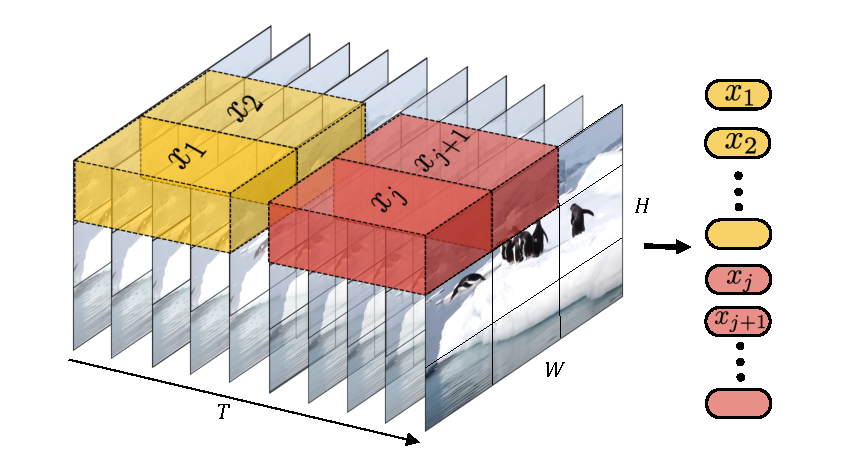
\includegraphics[width=0.9\linewidth]{figures/diagrams/Diagram-3.pdf}
    \caption{Tubelet embedding. We extract and linearly embed non-overlapping tubelets that span the spatio-temporal input volume. %
    }
    \vspace{-3mm}
    \label{fig:tokenizer_3d}
\end{figure}
An alternate method, as shown in Fig.~\ref{fig:tokenizer_3d}, is to extract non-overlapping, spatio-temporal ``tubes'' from the input volume, and to linearly project this to $\mathbb{R}^d$.
This method is an extension of ViT's embedding to 3D, and corresponds to a 3D convolution.
For a tubelet of dimension $t \times h \times w$, $n_t = \floor{\frac{T}{t}}$, $n_h = \floor{\frac{H}{h}}$ and $n_w = \floor{\frac{W}{w}}$, tokens are extracted from the temporal, height, and width dimensions respectively.
Smaller tubelet dimensions thus result in more tokens which increases the computation. Intuitively, this method fuses spatio-temporal information during tokenisation, in contrast to ``Uniform frame sampling'' where temporal information from different frames is fused by the transformer.


\subsection{Transformer Models for Video}
\label{sec:method_video_models}

As illustrated in Fig.~\ref{fig:teaser}, we propose multiple transformer-based architectures.
We begin with a straightforward extension of ViT~\cite{dosovitskiy_iclr_2021} that models pairwise interactions between all spatio-temporal tokens, and then develop more efficient variants which factorise the spatial and temporal dimensions of the input video at various levels of the transformer architecture.

\paragraph{Model 1: Spatio-temporal attention}
This model simply forwards all spatio-temporal tokens extracted from the video, $\mathbf{z}^{0}$, through the transformer encoder.
We note that this has also been explored concurrently by~\cite{bertasius_arxiv_2021} in their ``Joint Space-Time'' model.
In contrast to CNN architectures, where the receptive field grows linearly with the number of layers, each transformer layer models all pairwise interactions between all spatio-temporal tokens, and it thus models long-range interactions across the video from the first layer.
However, as it models all pairwise interactions, Multi-Headed Self Attention (MSA)~\cite{vaswani_neurips_2017} has quadratic complexity with respect to the number of tokens.
This complexity is pertinent for video, as the number of tokens increases linearly with the number of input frames, and motivates the development of more efficient architectures next.%

\paragraph{Model 2: Factorised encoder}
\begin{figure}
    \vspace{-0.5\baselineskip}
    \centering
    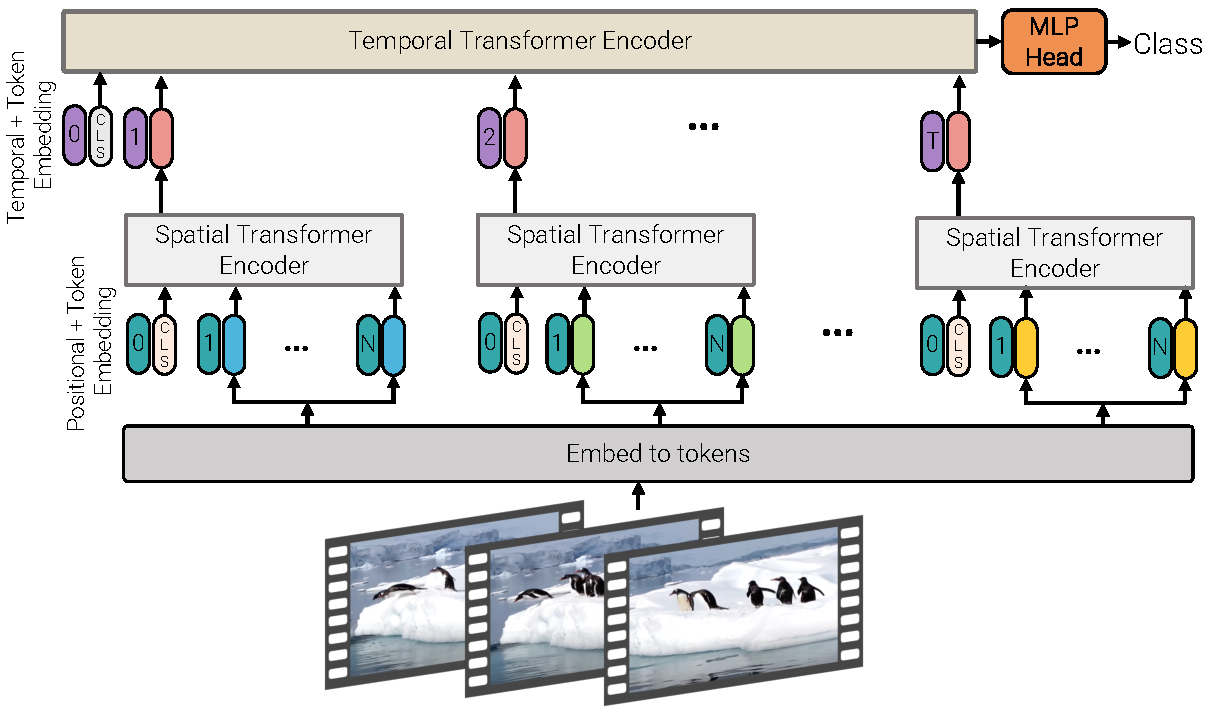
\includegraphics[width=1.0\linewidth]{figures/diagrams/ViViT_fac_1.pdf}
    \vspace{0.1em}
    \caption{
    	Factorised encoder (Model 2). 
    	This model consists of two transformer encoders in series: the first models interactions between tokens extracted from the same temporal index to produce a latent representation per time-index.
    	The second transformer models interactions between time steps.
    	It thus corresponds to a ``late fusion'' of spatial- and temporal information.
    }
    \vspace{-\baselineskip}
    \label{fig:factorised_encoder}
\end{figure}

As shown in Fig.~\ref{fig:factorised_encoder}, this model consists of two separate transformer encoders.
The first, spatial encoder, only models interactions between tokens extracted from the same temporal index. %
A representation for each temporal index, $h_i \in \mathbb{R}^d$, is obtained after $L_s$ layers: This is the encoded classification token, $z_{cls}^{L_s}$ if it was prepended to the input (Eq.~\ref{eq:tokens}), or a global average pooling from the tokens output by the spatial encoder, $\mathbf{z}^{L_s}$, otherwise.
The frame-level representations, $h_i$, are concatenated into $\mathbf{H} \in \mathbb{R}^{n_t \times d}$, and then forwarded through a temporal encoder consisting of $L_t$ transformer layers to model interactions between tokens from different temporal indices.
The output token of this encoder is then finally classified.

This architecture corresponds to a ``late fusion''~\cite{karpathy_cvpr_2014, simonyan_neurips_2014, wang_tsn_eccv_2016, neimark_arxiv_2021} of temporal information, and the initial spatial encoder is identical to the one used for image classification.
It is thus analogous to CNN architectures such as ~\cite{girdhar_neurips_2017, karpathy_cvpr_2014, wang_tsn_eccv_2016, zhou_trn_eccv_2018} which first extract per-frame features, and then aggregate them into a final representation before classifying them. %
Although this model has more transformer layers than Model 1 (and thus more parameters), it requires fewer floating point operations (FLOPs), as the two separate transformer blocks have a complexity of $\mathcal{O}({(n_h \cdot n_w)^2 + n_t^2)}$ compared to $\mathcal{O}((n_t \cdot n_h \cdot n_w)^2)$ of Model 1.


\paragraph{Model 3: Factorised self-attention}
\begin{figure}
    \vspace{-0.5\baselineskip}
    \centering
    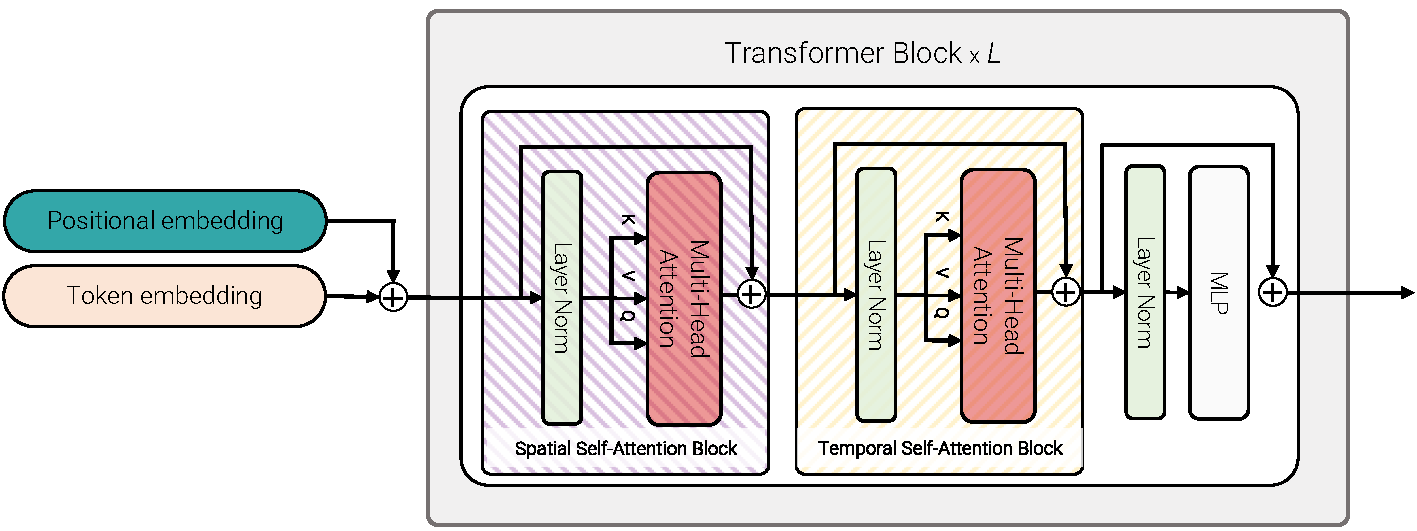
\includegraphics[width=1.0\linewidth]{figures/diagrams/ViViT_fac_2.pdf}
        \vspace{0.1em}
        \caption{ 
    	Factorised self-attention (Model 3).
    	Within each transformer block, the multi-headed self-attention operation is factorised into two operations (indicated by striped boxes) that first only compute self-attention spatially, and then temporally.
    }
    \label{fig:factorised_self_attention}
    \vspace{-\baselineskip}
\end{figure}

This model, in contrast, contains the same number of transformer layers as Model 1.
However, instead of computing multi-headed self-attention across all pairs of tokens, $\mathbf{z}^{\ell}$, at layer $l$, we factorise the operation to first only compute self-attention spatially (among all tokens extracted from the same temporal index), and then temporally (among all tokens extracted from the same spatial index) as shown in Fig.~\ref{fig:factorised_self_attention}.
Each self-attention block in the transformer thus models spatio-temporal interactions, but does so more efficiently than Model 1 by factorising the operation over two smaller sets of elements, thus achieving the same computational complexity as Model 2. %
We note that factorising attention over input dimensions has also been explored in~\cite{ho_arxiv_2019, weissenborn_iclr_2020}, and concurrently in the context of video by~\cite{bertasius_arxiv_2021} in their ``Divided Space-Time'' model.

This operation can be performed efficiently by reshaping the tokens $\mathbf{z}$ from $\mathbb{R}^{1 \times n_t \cdot n_h \cdot n_w \cdot d}$ to $\mathbb{R}^{n_t \times n_h \cdot n_w \cdot d}$ (denoted by $\mathbf{z}_s$) to compute spatial self-attention.
Similarly, the input to temporal self-attention, $\mathbf{z}_t$ is reshaped to $\mathbb{R}^{n_h \cdot n_w \times  n_t \cdot d}$.
Here we assume the leading dimension is the ``batch dimension''.
Our factorised self-attention is defined as
\begin{align}
\mathbf{y}_{s}^{\ell}    &= \msa(\lnorm(\mathbf{z}^{\ell}_s)) + \mathbf{z}^{\ell}_s \\
\mathbf{y}_{t}^{\ell}    &= \msa(\lnorm(\mathbf{y}^{\ell}_s)) + \mathbf{y}^{\ell}_s  \label{eq:factorised_self_att_temporal} \\
\mathbf{z}^{\ell + 1}  &= \mlp(\lnorm(\mathbf{y}_t^{\ell})) + \mathbf{y}_t^\ell.
\end{align}
We observed that the order of spatial-then-temporal self-attention or temporal-then-spatial self-attention does not make a difference, provided that the model parameters are initialised as described in Sec.~\ref{sec:method_initialisation}.
Note that the number of parameters, however, increases compared to Model 1, as there is an additional self-attention layer (cf. Eq.~\ref{eq:selfattn}).
We do not use a classification token in this model, to avoid ambiguities when reshaping the input tokens between spatial and temporal dimensions.

\paragraph{Model 4: Factorised dot-product attention}
\begin{figure}
    \centering
    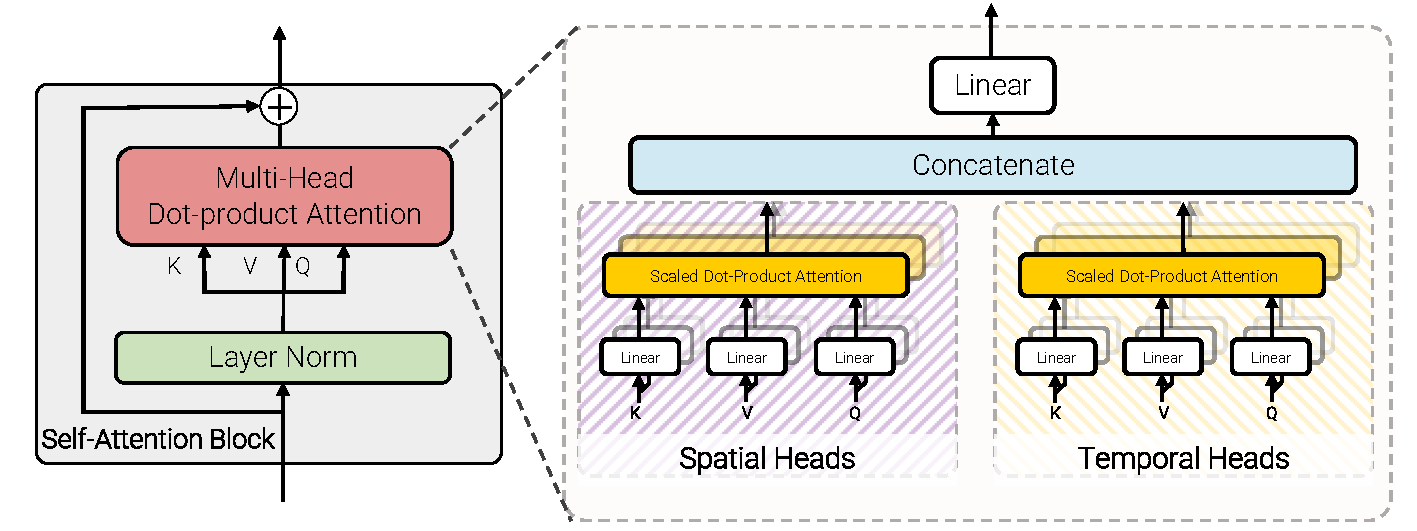
\includegraphics[width=1.0\linewidth]{figures/diagrams/ViViT_fac_3.pdf}
    \caption{Factorised dot-product attention (Model 4).
    For half of the heads, we compute dot-product attention over only the spatial axes, and for the other half, over only the temporal axis.
    }
    \label{fig:factorised_dot_product_attention}
    \vspace{-\baselineskip}
\end{figure}
Finally, we develop a model which has the same computational complexity as Models 2 and 3, while retaining the same number of parameters as the unfactorised Model 1.
The factorisation of spatial- and temporal dimensions is similar in spirit to Model 3, but we factorise the multi-head dot-product attention operation instead (Fig.~\ref{fig:factorised_dot_product_attention}).
Concretely, we compute attention weights for each token separately over the spatial- and temporal-dimensions using different heads.
First, we note that the attention operation for each head is defined as
\begin{align}
\attention(\mathbf{Q}, \mathbf{K}, \mathbf{V}) = \softmax\left(\frac{\mathbf{Q} \mathbf{K}^\top}{\sqrt{d_k}} \right) \mathbf{V}. \label{eq:selfattn}
\end{align}
In self-attention, the queries $\mathbf{Q} = \mathbf{X} \mathbf{W}_q$, keys $\mathbf{K} = \mathbf{X} \mathbf{W}_k$, and values $\mathbf{V}= \mathbf{X} \mathbf{W}_v$ are linear projections of the input $\mathbf{X}$ with $\mathbf{X}, \mathbf{Q}, \mathbf{K}, \mathbf{V} \in \mathbb{R}^{N \times d}$. 
Note that in the unfactorised case (Model 1), the spatial and temporal dimensions are merged as $N = n_t \cdot n_h \cdot n_w$.

The main idea here is to modify the keys and values for each query to only attend over tokens from the same spatial- and temporal index by constructing $\mathbf{K}_s, \mathbf{V}_s \in \mathbb{R}^{n_h \cdot n_w \times d}$ and $\mathbf{K}_t, \mathbf{V}_t \in \mathbb{R}^{n_t \times d}$, namely the keys and values corresponding to these dimensions. Then, for half of the attention heads, we attend over tokens from the spatial dimension by computing $\mathbf{Y}_s = \attention(\mathbf{Q}, \mathbf{K}_s, \mathbf{V}_s)$, and for the rest we attend over the temporal dimension by computing $\mathbf{Y}_t = \attention(\mathbf{Q}, \mathbf{K}_t, \mathbf{V}_t)$.
Given that we are only changing the attention neighbourhood for each query, the attention operation has the same dimension as in the unfactorised case, namely $\mathbf{Y}_s, \mathbf{Y}_t \in \mathbb{R}^{N \times d}$. 
We then combine the outputs of multiple heads by concatenating them and using a linear projection~\cite{vaswani_neurips_2017}, 
$\mathbf{Y} = \concat(\mathbf{Y}_s, \mathbf{Y}_t) \mathbf{W}_O$.






\subsection{Initialisation by leveraging pretrained models}
\label{sec:method_initialisation}

ViT~\cite{dosovitskiy_iclr_2021} has been shown to only be effective when trained on large-scale datasets, as transformers lack some of the inductive biases of convolutional networks~\cite{dosovitskiy_iclr_2021}. %
However, even the largest video datasets such as Kinetics~\cite{kay_arxiv_2017}, have several orders of magnitude less labelled examples when compared to their image counterparts~\cite{deng_cvpr_2009, kuznetsova_ijcv_2020, sun_iccv_2017}.
As a result, training large models from scratch to high accuracy is extremely challenging.
To sidestep this issue, and enable more efficient training we initialise our video models from pretrained image models.
However, this raises several practical questions, specifically on how to initialise parameters not present or incompatible with image models.
We now discuss several effective strategies to initialise these large-scale video classification models.

\paragraph{Positional embeddings}
A positional embedding $\mathbf{p}$ is added to each input token (Eq.~\ref{eq:tokens}).
However, our video models have $n_t$ times more tokens than the pretrained image model. As a result, we initialise the positional embeddings by ``repeating'' them temporally from $\mathbb{R}^{n_w \cdot n_h \times d}$ to $\mathbb{R}^{n_t \cdot n_h \cdot n_w \times d}$.
Therefore, at initialisation, all tokens with the same spatial index have the same embedding which is then fine-tuned.

\paragraph{Embedding weights, $\mathbf{E}$}
When using the ``tubelet embedding'' tokenisation method (Sec.~\ref{sec:method_input_encoding}), the embedding filter $\mathbf{E}$ is a 3D tensor, compared to the 2D tensor in the pretrained model,  $\mathbf{E}_{\text{image}}$. A common approach for initialising 3D convolutional filters from 2D filters for video classification is to ``inflate'' them by replicating the filters along the temporal dimension and averaging them~\cite{carreira_cvpr_2017, feichtenhofer_neurips_2016} as
\begin{equation}
\mathbf{E} = \frac{1}{t}[\mathbf{E}_{\text{image}}, \ldots, \mathbf{E}_{\text{image}}, \ldots, \mathbf{E}_{\text{image}}].
\end{equation}
We consider an additional strategy, which we denote as ``central frame initialisation'', where $\mathbf{E}$ is initialised with zeroes along all temporal positions, except at the centre $\floor{\frac{t}{2}}$,
\begin{equation}
\mathbf{E} = [\mathbf{0}, \ldots,  \mathbf{E}_{\text{image}}, \ldots, \mathbf{0}].
\label{eq:central_frame_init}
\end{equation}
Therefore, the 3D convolutional filter effectively behaves like ``Uniform frame sampling'' (Sec.~\ref{sec:method_input_encoding}) at initialisation, while also enabling the model to learn to aggregate temporal information from multiple frames as training progresses.

\paragraph{Transformer weights for Model 3}
The transformer block in Model 3 (Fig.~\ref{fig:factorised_self_attention}) differs from the pretrained ViT model~\cite{dosovitskiy_iclr_2021}, in that it contains two multi-headed self attention (MSA) modules.
In this case, we initialise the spatial MSA module from the pretrained module, and initialise all weights of the temporal MSA with zeroes, such that Eq.~\ref{eq:factorised_self_att_temporal} behaves as a residual connection~\cite{he_cvpr_2016} at initialisation.


